\documentclass[runningheads]{llncs}

%---- Codierung----%
\usepackage[utf8]{inputenc} 
%\usepackage[T1]{fontenc}
\usepackage{graphicx}
%\usepackage{url}
\usepackage{llncsdoc}
%----- Mathematischer Zeichenvorrat---%
%\usepackage{amsmath}
%\usepackage{amssymb}
%\usepackage{enumerate}
\usepackage{proof}
\usepackage{mathpartir}
% fuer die aktuelle Zeit 
%\usepackage{scrtime}
%\usepackage{listings}
%\usepackage{subfigure}
\usepackage{hyperref}

%referenzieren von Abbildungen
\usepackage[figure]{hypcap}
\setcounter{tocdepth}{3}
\setcounter{secnumdepth}{3}

% Syntax highlighting von Java Code
\usepackage{listings}
\usepackage{color}
 
\definecolor{dkgreen}{rgb}{0,0.6,0}
\definecolor{gray}{rgb}{0.5,0.5,0.5}
\definecolor{mauve}{rgb}{0.58,0,0.82}

\lstset{frame=tb,
  language=Java,
  aboveskip=3mm,
  belowskip=3mm,
  showstringspaces=false,
  columns=flexible,
  basicstyle={\small\ttfamily},
  numbers=left,
  numberstyle=\tiny\color{gray},
  keywordstyle=\color{blue},
  commentstyle=\color{dkgreen},
  stringstyle=\color{mauve},
  breaklines=true,
  breakatwhitespace=true,
  tabsize=3,
  escapechar=@
}
 
\usepackage{graphicx}
\begin{document}

\mainmatter
\title{Taint Analyse für Android Apps} 
\titlerunning{Taint Analyse für Android Apps}
\author{Thomas Czogalik}
\authorrunning{Desaster in der Software-Sicherheit (WiSe15/16)}
\institute{Betreuer: Simon Greiner}
\date{31.03.2016}
\maketitle

\section{Motivation} 
Computersysteme sind heutzutage in nahezu allen Bereichen unseres Lebens intigriert. Datenlecks können deshalb fatale folgen haben. Besonders Smartphones verwalten und verarbeiten viele vertauliche und private Daten und komunizieren dabei oft mit der Außenwelt. Im Februar 2015 befanden sich im Google Play Store ca. 1.4 Millionen Apps (\ref{fig:playstore}). Diese Apps sind jedem zugänglich, der auf seinem mobilen Gerät das Betriebssystem Android installiert hat. Bei so einer großen Anzahl Apps bietet der Google Play Store eine große Angriffsfläche für Angreifer die Datenlecks ausnutzen. \\
Betrachten wir den folgenden Ausschnitt aus einem Java Programm in Abbildung \ref{fig:sql_code}. In Zeile \ref{sql:connection} wird zunächst eine Verbindung zu einer Datenbank hergestellt. In den nächsten beiden Zeilen \ref{sql:createStmt} und \ref{sql:createBr} werden ein \emph{Statement} Objekt und ein \emph{BufferdReader} Objekt erstellt. In Zeile \ref{sql:name} wird eine Benutzereingabe eingelesen und dem String \emph{name} zugewiesen. In Zeile \ref{sql:sql} wird der String \emph{name} in einen vorbereiteten SQL String eingesetzt. Schließlich wird in Zeile \ref{sql:sink} das Statement mit dem String \emph{sql} ausgeführt. 
\\Durch folgende Benutzereingabe: \emph{foo; DROP TABLE users} kann die Datenbank \emph{users} gelöscht werden. Es können aber auch mit einem beliebigen SELECT Statement Daten aus der Datenbank geholt werden. 
\\Durch eine Überprüfung der Benutzereingabe hätte man diesen Fehler vermeiden können. Es ist aber nicht immer so einfach Datenlecks im Code zu finde. 
Deshalb wäre es hilfreich, wenn man den Fluss sensitiver Daten nachvollziehen könnte. Dies ist mithilfe einer Taint Analyse möglich. \\
Im folgenden wird zunächst auf die Grundlagen der Taint Analyse eingegangen um sie dann anschließend Formal darzustellen [\ref{sec:taintAnalyse}]. Außerdem werden Eigenschaften für die Taint Analyse vorgestellt, die zur einer besseren Präzision führen [\ref{sec:precision}]. Im Anschluß wird auf die Probleme bei Android eingegangen die bei einer Taint Analyse auftretten [\ref{sec:android}]. Schließlich wird FlowDroid vorgestellt, statische Taint Analyse für Android Apps [\ref{sec:flowdroid}].
 
\begin{figure}[htp]
\centering
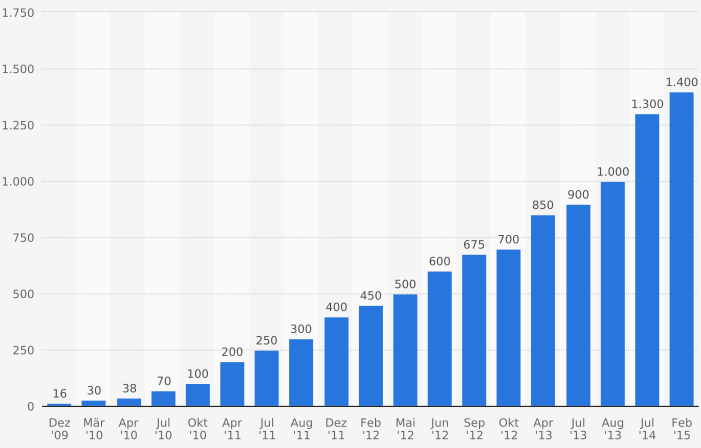
\includegraphics[scale=0.60]{img/playstore.png}
\caption{Anzahl der verfügbaren Apps im Google Play Store von Dezember 2009 bis Februar 2015 (in 1.000), aus \cite{playstore}}
\label{fig:playstore}
\end{figure} 

\begin{figure}
\lstinputlisting[language=Java]{code/sql_example.java}
\caption{Beispiel bei dem SQL Injections möglich sind}
\label{fig:sql_code}
\end{figure}

\section{Taint Analyse}\label{sec:taintAnalyse}
Die Taint Analyse ist eine Datenflussanalyse. Man unterscheidet zwischen statischer und dynamischer Taint Analyse. Bei einer statischen Analyse wird der Quelltext einer Reihe formaler Prüfungen unterzogen. Der Vorteil dabei ist, dass das Kompilat nicht ausgeführt werden muss, im Gegensatz zur dynamischen Analyse, die ein laufendes Programm voraussetzt. Dies ist hilfreich, da heutige Malware erkennen kann ob sie überwacht wird und ihr Verhalten der Situation anpasst. \\
Im folgenden wird sich auf die statische Taint Analyse beschränkt.\\\\
Die Taint Analyse nimmt zunächst an, dass jede von außen veränderbare Variable ein Sicherheitsrisiko birgt. Ihr Ziel ist es, die Software gegen externe Angriffe, sowie interne Risiken abzusichern. Dazu sucht die Taint Analyse nach Datenflüssen von möglichen tainted Sources zu einem Sink. Als Source wird eine Funktion bezeichnet, die Quelle sensitiver Daten ist. Ein Sink ist eine Funktion, die Daten möglicherweiese an nicht vertrauenswürdige Beobachter weitergibt. Welche Funktionen im einzelnen Sources und Sinks sind, muss vor dem ausführen der Taint Analyse spezifiziert werden. In dem Beispiel aus Abbildug \ref{fig:sql_code} wäre die Funktion \emph{readLine()} eine Source, da Daten von außen eingeführt werden (Benutzereingabe) und die Funktion \emph{executeQuery(sql : String)} ein Sink, da hier möglicherweise sensitive Daten weitergegeben werden.
\section{Formal}
Im Folgendem wird die Taint Analyse mithilfe von Schlussregeln in Abbildung \ref{fig:schlussregeln} formalisiert. Eine Schlussregel besteht aus einer Menge von Prämissen, die über dem Schlussstrich stehen und einer Konklusion die darunter steht. Wenn die Prämissen alle wahr sind folgt die Konklusion. \\
Die Regeln setzten sich aus den folgenden Prämissen zusammen:\\\\
\begin{tabular}{ll}
	\textbf{Prämisse}			& \textbf{Bedeutung}\\
	\emph{src(m,so)}			& Dem Parameter \emph{m} werden tainted Daten aus einer Source mit \\ 
								& dem Namen \emph{so} zugewiesen\\
	\emph{sink(m,si)} 			& Der Parameter \emph{m} wird in einen Sink mit dem Namen \emph{si} \\
								& übergeben\\
	\emph{tainted(o,so)} 		& Der Objektrepräsentant \emph{o} wird durch eine Source mit dem \\
								& Namen \emph{so} tainted\\
	\emph{flow(so,si)} 			& Es gibt einen Datenfluss von einer Source mit dem Namen \emph{so} zu\\
								& einem Sink mit Namen \emph{si}\\
	\emph{transfer(m,n)} 		& Es werden Daten von Parameter \emph{m} zu Parameter \emph{n} übertragen\\
	\emph{m $\rightarrow$ o} 	& Die Variable \emph{m} zeigt auf einen Objektrepräsentanten \emph{o}
\end{tabular}\\\\\\
Die Namen der Sources und Sinks stammen jeweils aus einem Source-Label-Set, bzw. einem Sink-Label-Set. Diese Sets enthalten alle Sources und Sinks die für die jeweilige Taint Analyse spezifiziert wurden. Als Objektrepräsentant wird ein Objekt im Sinne der Analyse bezeichnet.\\
Die erste Regel ist die SOURCE Regel. Sie beschreibt die Zuweisung von tainted Daten durch eine Source. Die SOURCE Regel setzt sich aus den Prämissen \emph{src(m,l)} und \emph{m $\rightarrow$ o} zusammen. Wenn diese beiden Prämissen wahr sind folgt die Konklusion \emph{tainted(o,l)}. \\
Möchte man die SOURCE Regel auf das Beispiel aus Abbildung \ref{fig:sql_code} anwenden, muss man zunächst die Sources und Sinks definieren und diese in das jeweilige Set eintragen. In das Source-Label-Set wird die Funktion \emph{readline()} aus Zeile \ref{sql:name} eingetragen, da hier durch die Benutzereingabe potentiell gefährliche Daten reinkommen können. In das Sink-Label-Set wird die Funktion \emph{executeQuery(s : String)} eingetragen, da hier möglicherweise tainted Daten weitergegeben werden können. Die SOURCE Regel wird in Zeile \ref{sql:name} den String \emph{name} als tainted durch die Source \emph{readLine()} markieren, da die beiden Prämissen wahr sind.\\
Die zweite Regel TRANSFER beschreibt die Übertragung von tainted Daten. Sie besteht aus den Prämissen \emph{tainted($o_1$,l)}, \emph{m $\rightarrow$ $o_1$} ,\emph{n $\rightarrow$ $o_2$} und \emph{transfer(m,n)}. Wenn alle Prämissen wahr sind, dann folgt die Konklusion \emph{tainted($o_2$,l)}.\\
Die TRANSFER Regel wir in dem Beispiel aus Abbildung \ref{fig:sql_code} in Zeile \ref{sql:sql} angewendet, da hier Daten vom String \emph{name} zum String \emph{sql} übertragen werden. Da auch hier alle Prämissen der TRANSFER Regel erfüllt sind, wird der String \emph{sql} auch als tainted markiert. \\
Die letzte Regel SOURCE beschreibt den Datenfluss von tainted Daten zu einem Sink. Sie besteht aus den Prämissen \emph{tainted(o,so)}, \emph{m $\rightarrow$ o} und \emph{sink(m,si)}. Sind alle Prämissen wahr, dann folgt die Konklusion \emph{flow(so,si)} und der Sink \emph{si} wird als tainted markiert. 
Die SOURCE Regel wird in dem Beispiel aus Abbildung \ref{fig:sql_code} in Zeile \ref{sql:sink} angewendet, da hier der String \emph{sql} dem Sink \emph{executeQuery} übergeben wird. Auch hier sind alle Prämissen der SOURCE Regel erfüllt und somit folgt die Konklusion und der Sink \emph{executeQuery} wird als tainted markiert.\\
Mit diesen drei Regeln und Fixpunktiteration kann man eine Taint Analyse durchführen.
\begin{figure}[t]
\begin{mathpar}
\infer[(SOURCE)] {tainted(o, l)}{src(m,l)\\ m \rightarrow o}\\\\
\infer[(TRANSFER)] {tainted(o_2, l)}{tainted(o_1,l)\\ m \rightarrow o_1 \\ n \rightarrow o_2 \\ transfer(m,n)}\\\\
\infer[(SOURCE)] {flow(so, si)}{tainted(o,so)\\ m \rightarrow o \\ sink(m,si)} 
\end{mathpar}
\caption{Schlussregeln für die Taint Analyse}
\label{fig:schlussregeln}
\end{figure}

\section{Sanitization}
Mithilfe von Sanitization Funktionen lassen sich Code Injections verhindern. Als Code Injection bezeichnet man das ausnutzen eines Programmfehlers indem man Code in das Program einschleust.
\\In Abbildung \ref{fig:sql_code} würde zum Beispiel die Funktion \emph{onlyLetters(s : String) : String} die Benutzereingabe als Parameter entgegen nehmen, alle nicht Buchstaben aus der Eingabe entfernen und einen String zurückgeben, der nur aus Buchstaben besteht. Einige Programmiersprachen bieten solche Säuberungsfunktionen an. PHP hat zum Beispiel die Funktion \emph{htmlentities}. Diese Funktion konvertiert Zeichen, die in HTML besondere Bedeutung haben in ihre HTML Instanzen. Aus dem Zeichen '\textless' wird '\&lt;'.\\
Eine Taint Analyse die Sanitization unterstützt, hat den Vorteil, dass gesäuberte Daten nicht länger als tainted angesehen werden und nicht mehr als tainted in der Analyse verbreitet werden.

\section{Präzision}\label{sec:precision}
Eine gute Analyse sollte in der Lage sein keine false-positives zu finden. Dadurch wird zum einen die manuelle Aussortierung dieser durch den Benutzer vermieden und zum anderen die Präzision der Analyse erhöht. Dabei ist ein false-positive ein Ergebnis das anzeigt, dass eine bestimmte Voraussetzung erfüllt ist, obwohl dies nicht der Fall ist. Eine Analyse die eine oder mehrere der folgenden Eigenschaften implementiert hat den Vorteil, dass weniger false-positives gefunden werden.

\subsection{Fluss-Sensitivität}
Eine Analyse die Fluss-Sensitiv ist, beachtet die Reihenfolge der Programmbefehle.
In Abbildung \ref{fig:fluss_code} wird dem String \emph{s} in Zeile \ref{flow:s} zunächst ein harmloser Wert zugewiesen. Danach wird dieser String in Zeile \ref{flow:sink} einem Sink übergeben. Im Anschluss werden in Zeile \ref{flow:source} dem String \emph{s} tainted Daten aus einem Source zugewiesen. \\
Eine Fluss-Sensitive Analyse wird den Sink in Zeile \ref{flow:sink} nicht als tainted markieren, da sie die Reihenfolge der Programmbefehle beachtet. 

\begin{figure}
\lstinputlisting[language=Java]{code/flow_sensitive_example.java}
\caption{Fluss-Sensitivität}
\label{fig:fluss_code}
\end{figure}

\subsection{Kontext-Sensitivität}
Ist eine Analyse Kontext-Sensitiv, beachtet sie den Kontext des Aufrufs. Dies bedeutet, dass eine solche Analyse zu dem Aufrufer einer Funktion zurück springen kann und somit den genauen Funktionsaufrufer bestimmen kann, während eine Analyse die nicht Kontext-Sensitiv ist alle möglichen Aufrufer berücksichtigen muss.
In Abbildung \ref{fig:context_code} werden den beiden Strings \emph{s1} und \emph{s2} die Rückgabe der Funktion \emph{id(s : String) : String} zugewiesen. Die Funktion \emph{id} ist dabei die Identitätsfunktion. Nun wird \emph{id} einmal in Zeile \ref{context:s1} mit tainted Daten ausgeführt und \emph{s1} zugewiesen und noch einmal in Zeile \ref{context:s2} mit einem harmlosen String und \emph{s2} zugewiesen. Schließlich wird \emph{s2} dem sink in Zeile \ref{context:sink} übergeben. Eine Kontext-Sensitive Analyse kann hier zwischen den beiden Aufrufen in Zeile \ref{context:s1} und \ref{context:s2} unterscheiden und wird den Sink in Zeile \ref{context:sink} nicht als tainited markieren.
 
\begin{figure}
\lstinputlisting[language=Java]{code/context_sensitive_example.java}
\caption{Kontext-Sensitivität}
\label{fig:context_code}
\end{figure}

\subsection{Objekt-Sensitivität}
Die Objekt-Sensitivität ist ein Subtyp der Kontext-Sensitivität. Eine Objekt-Sensitive Analyse beachtet nämlich den Kontext des aufrufenden Objekts. Das heißt, dass zu dem Objekt zurück gesprungen werden kann, dass eine Methode aufruft.
In Abbildung \ref{fig:object_code} werden zunächst zwei \emph{Foo} Objekte \emph{o1} und \emph{o2} erstellt. Die Klasse \emph{Foo}  besteht aus einem String mit Namen \emph{value} und einer \emph{getValue() : String} Methode, die \emph{value} zurückgibt. In Zeile \ref{object:o1} und \ref{object:o2} wird \emph{o1} ein harmloser String übergeben und \emph{o2} tainted Daten aus einer Source. Im Anschluss wird in Zeile \ref{object:sink} die Funktion \emph{getValue} auf \emph{o1} aufgerufen und der Rückgabewert einem Sink übergeben. Eine Objekt-Sensitive Analyse kann zwischen den beiden Objekten \emph{o1} und \emph{o2} unterscheiden und markiert den Sink in Zeile \ref{object:sink} nicht als tainted. 

\begin{figure}
\lstinputlisting[language=Java]{code/object_sensitive_example.java}
\caption{Objekt-Sensitivität}
\label{fig:object_code} 
\end{figure}

\subsection{Feld-Sensitivität}
Eine Feld-Sensitive Analyse kann Felder einer Klasse einzelnd betrachten. Macht eine Analyse dies nicht, werden die Felder zu ihrem Basis Objekt zurückgeführt.
In Abbildung \ref{fig:field_code} wird in Zeile \ref{field:o} zunächst ein \emph{Foo} Objekt \emph{o} erstellt. Die Klasse \emph{Foo} enthält hier 2 Felder \emph{field1} und \emph{field2}. In Zeile \ref{field:f1} und \ref{field:f2} wird \emph{field1} ein harmloser String zugewiesen während \emph{field2} tainted Daten zugewiesen werden. Schließlich wird \emph{field1} in einen Sink in Zeile \ref{field:sink} übergeben. Bei einer Feld-Sensitiven Analyse wird hier der Sink nicht als tainted markiert.

\begin{figure}
\lstinputlisting[language=Java]{code/field_sensitive_example.java}
\caption{Feld-Sensitivität}
\label{fig:field_code}
\end{figure}

\section{Android}\label{sec:android}
Android ist sowohl ein Betriebssystem als auch eine Software-Platform für mobile Geräte. Es bietet Entwicklern eine Schnittstelle an, um auf verschiedene Systemfunktionalitäten des mobilen Gerätes zuzugreifen. Der Nutzerstandort ist zum Beispiel eine solche Funktionalität. Der Entwickler muss die von ihm genutzte Funktionalität in die \emph{AndroidManifest.xml} eintragen. Der Benutzer, der die App installieren möchte muss dieser die Berechtigung geben auf diese Funktionalitäten zugreifen zu dürfen. Oft werden zu viele Berechtigungen gefordert. Dies geschieht entweder aus Unkenntnis oder mit bösen Absichten. Außerdem sind viele Berechtigungen zu mächtig und können ausgenutzt werden. Eine social-network App zum Beispiel, möchte die Berechtigung\\\emph{android.permission.READ\_CONTACTS} um neue Freunde anhand der Email Adresse vorschlagen zu können. Sie kann aber mit dieser Berechtigung auch Telefonnummern und sonstige Kontaktdaten auslesen, auch wenn der Kontakt nicht bei dem Dienst angemeldet ist. Dies kann ausgenutzt werden.\\
Um dem entgegenzuwirken kann man die Datenflüsse einer Android App mithilfe der Taint Analyse analysieren. \\\\
Eine Android App kann aus vier Arten von Komponenten bestehen.\\\\
\begin{tabular}{ll}
	Activity & Einzelner Screen, der für den Benutzer sichtbar ist\\
	Service & Eine Aktion die im Hintergrund abläuft\\
	Content Provider & Ist zuständig für das Lesen und Speichern von Daten\\
	Broadcast Reciever & Wartet auf ein globales Ereignis und führt eine vordefinierte \\
	& Aktion aus\\\\
\end{tabular}
Da eine Android App aus einer beliebigen Zusammensätzung dieser Komponenten bestehen kann, zum Beispiel drei Activities und einem Service, entstehen Schwierigkeiten für eine Taint Analyse. Zunächst hat eine Android App keine zentrale \emph{main} Methode, sondern kann aufgrund der verschiedenen Komponenten mehrere Einstiegspunkte haben. Es gibt zwar eine Haupt-Activity, aber welche Komponente als nächstes an die Reihe kommt ist im allgemeinen nicht bestimmbar, da diese von der Benutzereingabe abhängig sind. Außerdem haben die einzelnen Komponenten besonderes Verhalten. Sie können zum Beispiel gestartet und beendet werden oder angehalten werden, wenn der Speicher voll ist und fortgesetzt, wenn wieder Speicher frei ist. Somit entsteht ein komplizierter Lebenszyklus, mit dem die Taint Analyse umgehen muss, da tainted Daten zwischen den Komponenten hin und hergereicht werden können in beliebiger Reihenfolge und mit verschiedenem Verhalten der einzelnen Komponenten. 

\section{FlowDroid}\label{sec:flowdroid}
FlowDroid\footnote{\url{https://github.com/secure-software-engineering/soot-infoflow-android/wiki}} ist eine statische Taint Analyse. Sie ist Fluss-, Kontext-, Objekt- und Feld-Sensitiv. Zur Bestimmung der Sources und Sinks benutzt FlowDroid das Tool SuSi. SuSi ist ein machine-learning Tool, dass vollautomatisch den Android Source Code analysiert und eine Liste von Sinks und Sources generiert. Außerdem generiert FlowDroid vor der Taint Analyse einen präzisen Android Lebenszyklus.\\
Aufgrund der vielen möglichen Einstiegspunkte bei einer Android App, wird bei FlowDroid zunächst eine dummy-main-Methode erstellt. Diese Methode wird individuell für jede App erstellt. Die dummy-main enthält nur Teile des Lebenszyklus die auch auftreten können. Um diese zu identifizieren werden die XML Konfigurationsdateien und der Quellcode analysiert. Danach ruft die dummy-main-Methode nachheinander Teile des Zyklus auf. 
In Abbildung \ref{fig:cycle_code} ist eine Klasse \emph{LeakageApp}, die von \emph{Activity} erbt und die Methode \emph{onRestart} überschreibt. Außerdem ist die methode \emph{sendMessage} im Layout-XML definiert und in \ref{fig:cycle_code} implementiert. In Abbildung \ref{fig:cycle_dummy} ist die von FlowDroid generierte dummy-main-Methode zu sehen. Es werden nur die Teile des Lebenszyklus verwendet, die in dem Beispiel vorkommen, wie die Methoden \emph{onRestart} und \emph{sendMessage}, bzw. vom Betriebssystem für den Lebenszyklus der App gebraucht werden, wie \emph{onCreate}, \emph{onStart}, \emph{onResume}, \emph{onPause}, \emph{onStop} und \emph{onDestroy}.
\begin{figure}
\lstinputlisting[language=Java]{code/lifecycle_example.java}
\caption{Lebenszyklus Code Beispiel}
\label{fig:cycle_code}
\end{figure}

\begin{figure}[t]
\centering

\includegraphics[scale=1.2]{img/lifecycle.png}
\caption{Aktivitätsdiagramm für die dummy Methode aus Abbildung \ref{fig:cycle_code}}
\label{fig:cycle_dummy}
\end{figure} 


\section{Evaluation}
Für die Evaluierung von FlowDroid wurde die Testumgebung DroidBench \footnote{\url{https://github.com/secure-software-engineering/DroidBench}} verwenden. DroidBench enthielt zum damaliegen Zeitpunkt 39 kleine Test Apps. FlowDroid wurde mit den beiden komerziellen Analyse Tools \emph{App Scan} von IBM und \emph{Fortify SCA} von HP verglichen. \\
Es gab dabei folgende Test Kategorien:\\\\
\begin{tabular}{ll}
	\textbf{Kategorie} 				& \textbf{Beschreibung}\\
	Arrays and Lists 				& Umgang mit Arrays und Listen\\
	Callbacks 						& Umgang mit Callbacks, sowohl in XML\\
			 						& definiert als auch im Code\\
	Field and Object Sensitivity 	& Feld- und Objekt-Sensitive Tests\\
	Inter-App Communication 		& Umgang mit tainted Daten, die einer anderen \\
									& Activity übergeben werden\\
	Lifecycle 						& Umgang mit Methoden des Lebenszyklus\\
	General Java 					& Allgemeine Java Tests\\
	Miscellaneous Android Specific 	& Verschiedene Android spezifische Tests wie, \\
									& Passwort Feld Eingabe wird geleakt\\
\end{tabular}\\\\
In dem Evaluierungsbogen in Abbildung \ref{fig:eval} ist zu erkennen, dass FlowDroid in den Kategorien \emph{Callbacks} und \emph{Lifecycle} deutlich besser ist, als \emph{Fortify} und \emph{App Scan}. Dies ist auf die präzise Modelierung des Lebenszyklus zurückzuführen. FlowDroid findet aber auch nicht alle Fehler. In dem Test \emph{IntentSink1} findet FlowDroid den Fehler nicht, da in dem Test tainted Daten aus einer Komponente in die nächste übergeben werden und diese Komponente die Daten direkt wieder zurück schickt. FlowDroid verfolgt tainted Daten nur innerhalb von Komponenten. Deshalb findet FlowDroid den Fehler in diesem Test nicht. Auch in dem Test \emph{StaticInitialization1} findet FlowDroid den Fehler nicht. Hier liegt der Grund in dem von FlowDroid generierten Call-Graphen. Bei der Generierung geht FlowDroid davon aus, dass die komplette statische Initialisierung zu beginn stattfindet, was in diesem Testfall nicht der Fall ist.\\
Im Ergebniss ist FlowDroid aber deutlich besser als \emph{Fortify} und \emph{App Scan}. FlowDroid erzielt eine Präzision von 86\%, während \emph{Fortify} 81\% und \emph{App Scan} 74\% erreichen. Als Präzision wird hier das Verhältnis zwischen gefunden Fehlern und false-positives bezeichnet. Außerdem findet FlowDroid 93\% aller Fehler in den Testfällen während \emph{Fortify} 61\% und \emph{App Scan} nur 50\% aller Fehler finden. \\
Mit FlowDroid wurden zusätzlich die damals Top 500 Apps des Google Play Stores getestet. Dabei wurden in den meisten Apps ein Datenleck gefunden, die aber keine bösartigen Absichten erkennen liesen.\\
Außerdem wurden 1000 Malware Apps des VirusShare Projects analysiert. Es wurden pro App ca. zwei Datenlecks gefunden.\\
Das zeigt, dass FlowDroid sowohl Datenlecks finden kann die unabsichtlich entstehen, als auch solche die absichtlich in eine App eingebaut werden.

\begin{figure}[htp]
\centering 
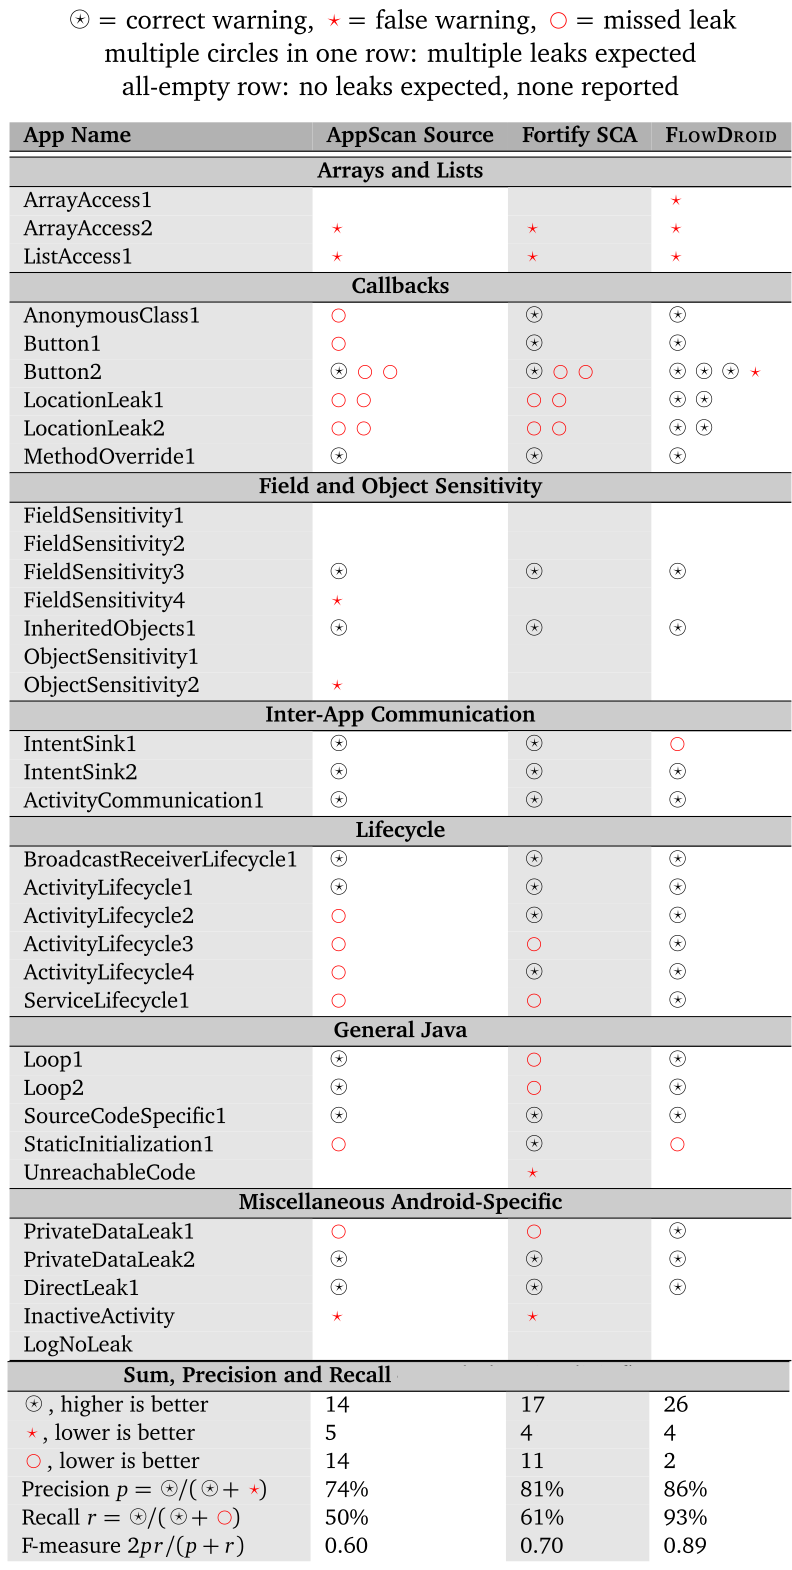
\includegraphics[scale=1]{img/evaluation.png}
\caption{DroidBench Evaluierung, aus \cite{technical}}
\label{fig:eval}
\end{figure} 
 
\section{Ausblick} 
FlowDroid macht vieles richtig, aber wie die Evaluierung gezeigt hat, findet FlowDroid noch nicht alle möglichen Datenlecks.\\ 
Zum Beispiel verfolgt FlowDroid tainted Daten nur innerhalb einer Komponente. Es sollte aber auch möglich sein, tainted Daten zwischen den Komponenten zu verfolgen. Dazu könnte ein Sink der einen Komponente gleichzeitig die Source der anderen Komponenten sein.\\
Außerdem hat FlowDroid keine Sanitization implementiert. Dies ist jedoch notwendig, damit der Programmierer auf gefundene Datenlecks reagieren und tainted Daten auch säubern kann. \\
Für die Zukunft wäre es auch wichtig, dass FlowDroid unterscheiden kann zwischen notwendigen und bösartigen Datenlecks. Eine Navigationsapp benötigt den Benutzerstandort. Eine Taschenlampen App jedoch nicht.\\
Schließlich wäre es auch hilfreich, wenn die Analyse für bestimmte Arten von Sinks und Sources einschränkbar wäre. Der Vorteil hierbei wäre, dass man sich bestimmte Datenflüsse näher anschauen könnte.

\section{Ergebnis}
In dieser Seminararbeit wurde die statische Taint Analyse vorgestellt und erklärt. Die Taint Analyse wurde mithilfe von Schlussregeln formalisiert und es wurden Analyseeigenschaften vorgestellt, mithilfe derer man eine Taint Analyse präziser machen kann. Außerdem wurde mit Sanitization ein Mechanismus vorgestellt mit dem man tainted Daten säubern kann und diese somit von der Taint Analyse nicht mehr als tainted weiterverbeitet werden. \\
Daraufhin wurde FlowDroid vorgestellt, eine statische Taint Analyse für Android Apps. Es wurde dargestellt wie FlowDroid mit den Schwierigkeiten umgeht, die bei einer Taint Analyse für Android Apps vorkommen. Außerdem wurde FlowDroid mit den beiden komerziellen Tools \emph{Fortify} von HP und \emph{App Scan} von IMB verglichen und hat gezeigt, dass es deutlich besser beim auffinden aller Datenlecks ist.\\
Schließlich wurden auch die Beschränkungen von FlowDroid aufgezeigt und mögliche Verbesserungen für die Zukunft der Analyse vorgestellt.
% Normaler LNCS Zitierstil
%\bibliographystyle{splncs}
 
\nocite{*}
\bibliographystyle{plain}
\bibliography{literatur}
\end{document}
